\documentclass[11pt]{article}
\usepackage{graphicx}
\usepackage[margin=2.5cm]{geometry}
\usepackage{tikz}
\usepackage{indentfirst}
\usepackage{tabularx}
\usepackage[portuguese]{babel}

\graphicspath{{./images/}}

\def\checkmark{\tikz\fill[scale=0.4](0,.35) -- (.25,0) -- (1,.7) -- (.25,.15) -- cycle;} 
\setlength{\parskip}{0.5em}

\begin{document}
	\begin{titlepage}
	\begin{center}
		
\includegraphics[width=0.6\textwidth]{logo-isec}
		
		\vspace*{\fill}
		
		\Huge
		\textbf{Interação Pessoa-Máquina}
		
		\huge
		Avaliação da Interface de dispositivos
		
		\vspace{0.5cm}
		\LARGE
		2020 - 2021
		
		\vspace{1.5cm}
		
		\textbf{TheForgotten\\merlin-twist}
		
		\begin{figure}[h]
			
\includegraphics[width=0.5\textwidth]{boomer}
			\centering
			\caption{Homem irritado com o computador}
			\label{fig:angry-man}
		\end{figure}
		
		\vfill
		\vspace*{\fill}
		
		\normalsize
		Licenciatura de Engenharia Informática \\
		5 de março de 2021		
	\end{center}
\end{titlepage}
	
	\tableofcontents
	\pagebreak
	
	\large
	\section{Introdução}
	
	\normalsize
	Este trabalho consiste na análise de um conjunto de exemplos de interfaces encontradas no dia-a-dia, e a identificação de aspetos positivos e negativos na sua interação com o utilizador.
	
	O objetivo é encontrar 3 exemplo onde esteja presente interação com o utilizador:
	
	\begin{itemize}
		\item Um objeto ou situação do dia-a-dia que traduza uma má interação;
		\item Uma má interface acessível num dispositivo informático (computador,
		telemóvel, PDA, ..);
		\item Um exemplo onde exista uma boa (e de preferência, original) concepção
		da interação (de preferência num dispositivo informático).
	\end{itemize}
	
	\large
	\section{Má Interação}
	
	\normalsize
	\begin{figure}[h]
		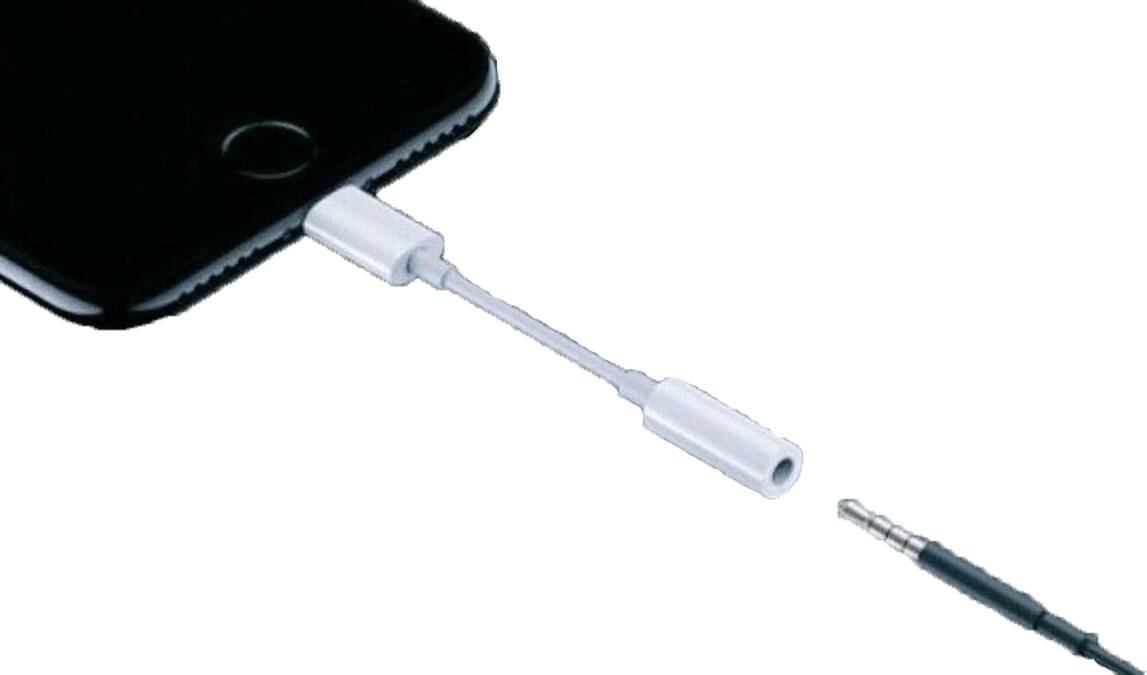
\includegraphics[width=0.6\textwidth]{dongle-life}
		\centering
		\caption{Exemplo de iPhone 7 com o dongle para aceitar 3.5mm}
		\label{fig:dongle-life}
	\end{figure}
	
	Um dos maiores exemplos de má interação presentes nos dias de hoje é a entrada de 3.5mm nos telemóveis (ou, melhor falando, a falta dela).
	
	Durante anos tornou-se standard a existência duma porta destas nos dispositivos móveis, chegando ao ponto de que todos os telemóveis tinham esta entrada e já nem era considerado um extra.
	
	Depois de tantos anos a normalizar esta entrada, a Apple aparece e anuncia o iPhone 7, o primeiro dispositivo sem uma entrada de 3.5mm, oferecendo como solução o uso de um dongle para os utilizadores poderem usufruir dos seus fones, iniciando assim a era da \textit{dongle life}, onde se torna a norma o uso de um dongle ou adaptador para quase tudo.
	
	E, com isto, aquilo que se tornou durante anos algo ordinário quase que desapareceu por completo num prazo de dois a três anos. Mas a parte que realmente mais incomoda é o facto de \textbf{nenhum} telemóvel topo de gama ter uma entrada de 3.5mm, mas os de baixa e média gama ainda terem, ou seja, de um modo geral, os telemóveis mais baratos possuem mais \textit{features}!
	
	A solução para este problema seria bastante simples: reintroduzir a entrada de 3.5mm nos dispositivos. Apesar do que os fabricantes dizem, isto ocupa muito pouco espaço no telemóvel, cabe perfeitamente e, bem implementado, não traz qualquer fragilidade ao dispositivo.
	
	\large
	\section{Má Interface}
	
	\normalsize
	\begin{figure}[h]
		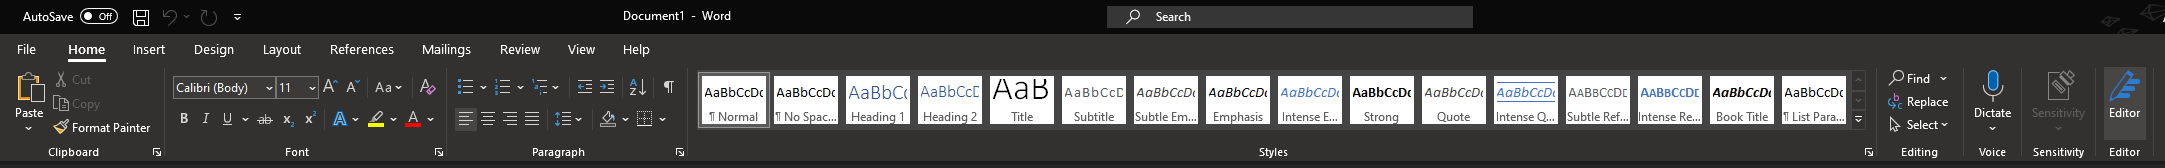
\includegraphics[width=1\textwidth]{word}
		\centering
		\caption{Exemplo de interface do Microsoft Word}
		\label{fig:word}
	\end{figure}
	
	Um excelente exemplo duma má interface é o Microsoft Word (em conjunto com todas as outras ferramentas pertencentes ao pacote Office e até o próprio Windows).
	
	Apesar de ter icones \textit{user friendly}, a interface está muito desordenada e densa. Acontece regularmente querer interagir com um botão e acabar por interagir com outro. Para além disto, alguns dos ícones são pouco intuitívos e, como não têm descrição, alguém que não esteja familiarizado com a ferramenta vai ter dificuldade a fazer o que pretende.
	
	Outro grande problema que esta ferramenta tem é o facto de que, dependendo da linguagem utilizada, os atalhos alteram-se, dificultando assim a vida de um utilizador experiente.
	
	Uma boa maneira de resolver este problema seria adicionar mais menus e mais específicos, facilitando não só a navegação pelos mesmo como também eliminando o problema de acidentalmente clicar onde não se quer, sendo que se há menos ícones por menu passará a existir também a possibilidade de adicionar uma descrição aos mesmos. Para o problema dos atalhos a solução é ainda mais simples: manter os atalhos de acordo com a norma utilizada em todo o lado.
	
	\large
	\section{Boa Interação}
	
	\normalsize
	\begin{figure}[h]
		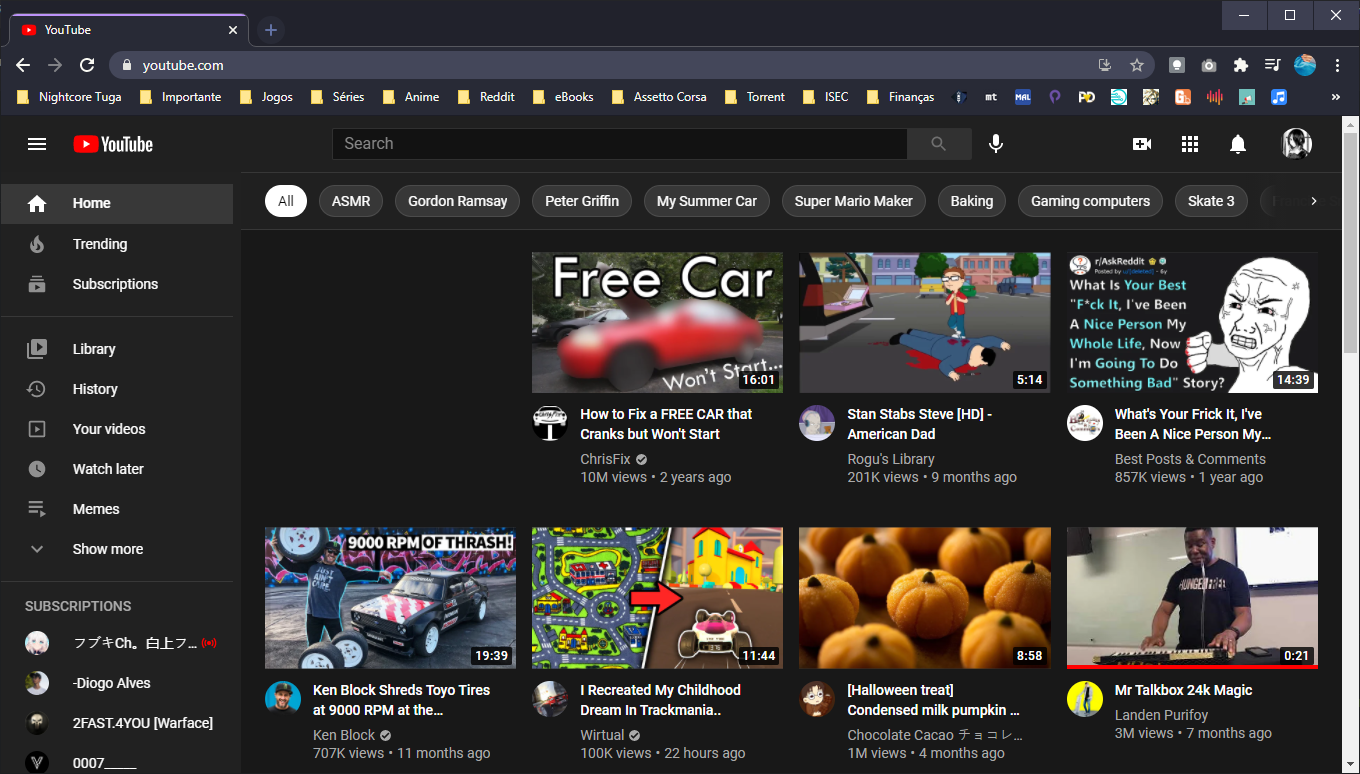
\includegraphics[width=0.9\textwidth]{youtube}
		\centering
		\caption{Exemplo de interface do YouTube}
		\label{fig:youtube}
	\end{figure}

	Tendo várias modificações ao longo dos anos, o YouTube é capaz de ser das melhores interfaces oferecidas atualmente.
	
	É simples, intuitíva, não é muito densa nem desorganizada, os ícones são fáceis de entender e possuem, na sua maioria, uma descrição simples mas eficaz do que cada botão representa.
	
	Dito em poucas palavras, achamos que o YouTube atingiu a perfeição em termos de interface, o que fornece uma simples e ótima interação para o utilizador. Uma boa maneira de ver o quão boa é a interação / interface fornecida é o facto de pessoas de todas as idades usarem o YouTube com facilidade, desde bebés quase recém-nascidos a idosos.
	
	Isto pode também ser visto na versão mobile da aplicação. Os menus são simples e pouco densos, e a interação com o utilizador é tão intuitiva que se faz o que a aplicação possibilita sem sequer se pensar no assunto.
	
	\large
	\section{Conclusão}
	
	\normalsize
	Este trabalho foi uma excelente maneira de despertar interesse nas interações pessoa-máquina.
	
	Para além disto, conseguimos concluir que, nos dias de hoje, más interfaces já não são tão comuns, principalmente devido ao facto de que agora existem normas. Por outro lado temos as más interações que, apesar de algumas já terem sido corrigidas, aparecem sempre novas que são tão más ou piores que as anteriores. 
	
	Mas, apesar de tudo, o mundo digital está de um modo geral cada vez mais intuitivo e utilizadores de todos os níveis de experiência conseguem facilmente interagir sem grande dificuldade com máquinas, ao contrário do que se verificava há uns anos.
	
	\pagebreak
	
	\large
	\section{Anexos}

	\normalsize
	\listoffigures
\end{document}